In this section the governing model equations for the x and y axes is Laplace transformed and put on transfer function. 

For the sake of repetition, the model expression for roll and pitch are as follows:
\begin{align}
m\Delta\ddot{x}_I&= -k_{th}({\overline{\omega}_1}^2+{\overline{\omega}_2}^2+{\overline{\omega}_3}^2+{\overline{\omega}_4}^2)\cos(\overline{\theta})\Delta\theta\\ \label{eq:model_x_transl}
m\Delta\ddot{y}_I&= k_{th}({\overline{\omega}_1}^2+{\overline{\omega}_2}^2+{\overline{\omega}_3}^2+{\overline{\omega}_4}^2)\cos(\overline{\phi})\cos(\overline{\theta})\Delta\phi \label{eq:model_y_transl}
\end{align} 
Laplace transforming \autoref{eq:model_x_transl} and \ref{eq:model_y_transl_y} yield:
\begin{align}
m x_1(s)s^2&=-k_{th}\cdot (\omega_1 ^2 + \omega_2 ^2 + \omega_3 ^2 + \omega_4 ^2) \theta\\
m y_1(s) s^2&= k_{th} (\omega_1 ^2 + \omega_2 ^2 + \omega_3 ^2 + \omega_4 ^2)\phi
\end{align}
It is desirable to have a transfer function where the input is the angle, as this is the output from the attitude controller that goes into the translational controller block. The output of the translational controller must be the velocity in the x and y axes respectively. \\
The transfer functions can now be written as:
\begin{align}
H_{x1}(s)&=\frac{x_1(s) s}{\theta}=\frac{-k_{th} (\omega_1 ^2 + \omega_2 ^2 + \omega_3 ^2 + \omega_4 ^2)}{m s}\label{eq:conHx}\\
H_{y1}(s)&=\frac{y_1(s) s}{\phi}=\frac{k_{th}(\omega_1 ^2 + \omega_2 ^2 + \omega_3 ^2 + \omega_4 ^2)}{m\cdot s}\label{eq:conHy}
\end{align}
\begin{where}
\va{H_{x1}}{is the plant for the translational roll}{1}
\va{H_{y1}}{is the plant for the translational pitch}{1}
\end{where}

From \autoref{eq:conHx} and \ref{eq:conHy} it is clearly seen that the two plants are similar but with different sign of the thrust coefficient. The controller design will be carried out for the translational roll model and applied for the translational pitch model  afterwards.

The systems are first order systems, that has one pole in zero and no zeroes. This means the systems are marginally stable. The roll model expression,\autoref{eq:conHx}, is negative, which requires a negative controller gain to become positive. If this is not done, the controller gain will move the pole to the right half plane, making the system unstable. This is not the case for the pitch model expression, \autoref{eq:conHy}.  

Moreover the zero-pole makes them type 1 systems, which means no steady state error will be present in a step response. 
A proportional controller is considered sufficient, as it does not have to compensate for a steady state error. By increasing the absolute gain value the system will become faster, which is desirable. To determine how large the absolute gain can be without making the system unstable due to saturation issues, it is necessary to consider the bandwidth. \\ \\
The data from the Vicon room is transmitted with 100 Hz. This means the attitude controller must run with 50 Hz as maximum to ensure the controller is slower than the sensor data. A rule of thumb states that the bandwidth of the system shall be 25 times smaller than the attitude controller. The desired bandwidth of the translational roll controller is calculated as follows:
\begin{align}
BW=2\cdot \pi\cdot \frac{f_s}{25}=2\cdot \pi \frac{50}{25}=12.57\label{eq:bw_X}
\end{align}
\begin{where}
\va{BW}{is the bandwidth of the plant}{rad \cdot s^{-1}}
\va{f_s}{is the sampling frequency of the plant}{Hz}
\end{where}

From \autoref{eq:bw_X} it is known, that the ideal bandwidth of the system is 12.57 rad/s. 
\begin{figure}[H]
	\centering
	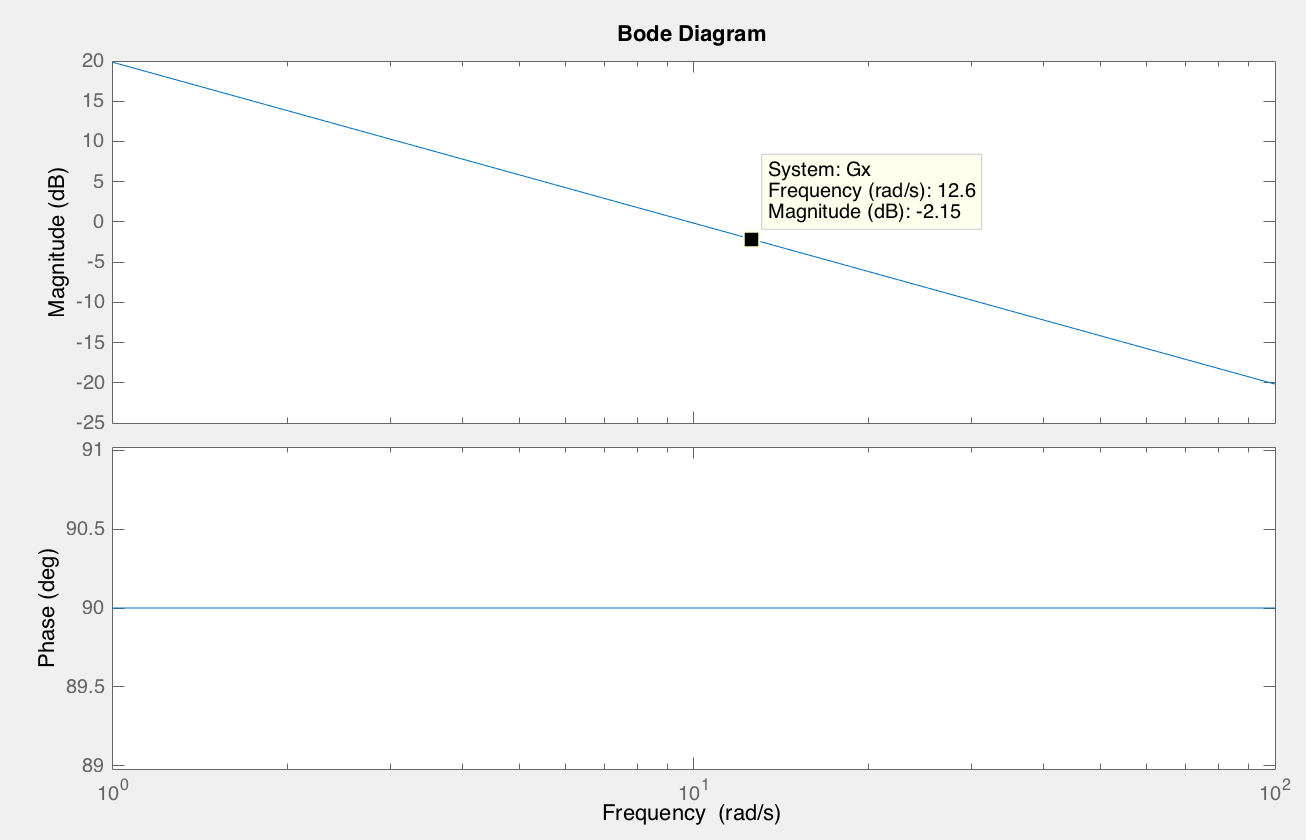
\includegraphics[width=0.7\textwidth]{figures/bode_x.png}
	\caption{Bodeplot of the plant, with the bandwidth of 12.6 rad/s displayed.}\label{fig:bode_x}
\end{figure}
The bodeplot in \autoref{fig:bode_x} reveals that the magnitude is -2.15 dB at 12.6 rad/s and must be lowered by 0.85 dB. 

The gain of the P-controller is found to be: 
\begin{align}
C_{x,y}=10^{\frac{-0.85}{20}}=0.907\\
\end{align}

The step response for the designed controller can be seen in \autoref{fig:step_x}
\begin{figure}[H]
	\centering
	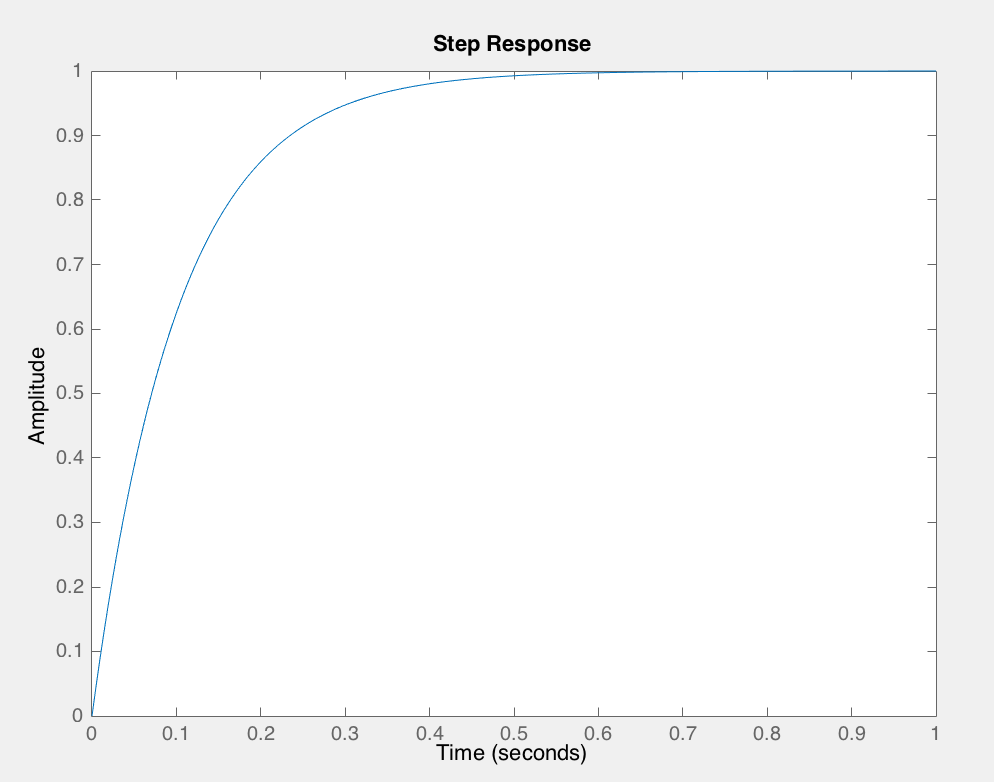
\includegraphics[width=0.8\textwidth]{figures/step_x.png}
	\caption{Step response for P-controller with a gain of -0.907 and 0.907 for x and y respectively.}\label{fig:step_x}
\end{figure}
When examining \autoref{fig:step_x}it is seen that, as expected,there is no steady state error. The system settles at 0.41 seconds and has a rise time of 0.12 seconds. Both settling time and rise time is within the requirements. As it is a first order system, there is no overshoot and it can therefore be concluded that the P-controller meets all requirements.
\\
\\
Before it can be implemented and tested on the quadcopter, it needs to be discretized. As it is P-controllers, it simply means to encounter the sampling rate. The discretized controllers are presented along with the continuous controller in \fxnote{make graph}.
\\ \\
  
%\subsubsection*{Pitch translational controller}
%The roll and pitch translational models are very similar and will therefore be designed similarly. The design procedure will be the same as for the translational roll controller.\\

% 
%The desired bandwidth is 12,57 rad/s as derived in \autoref{eq:bw_X}. 
%\begin{figure}[H]
%	\centering
%	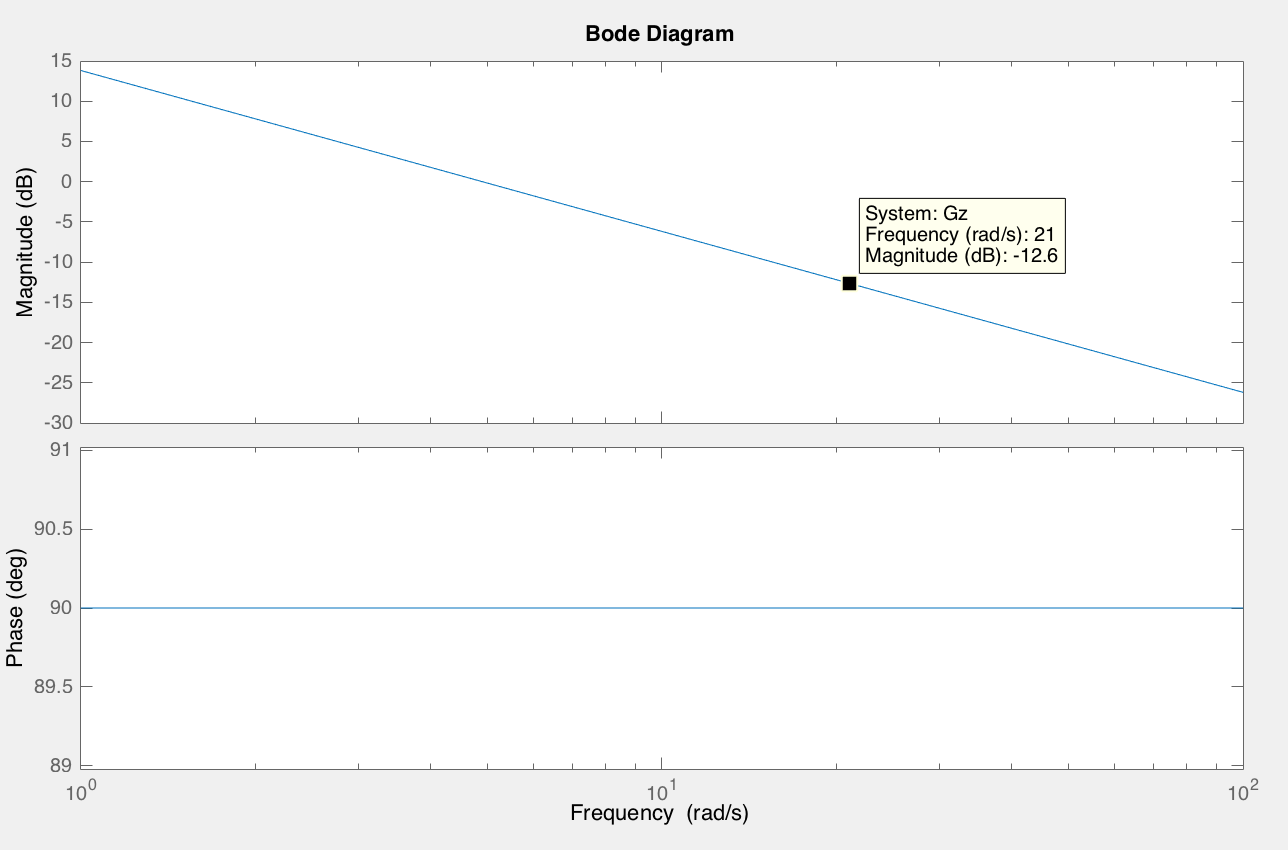
\includegraphics[width=0.7\textwidth]{figures/bode_y.png}
%	\caption{Bode plot of the plant with the 12.6 bandwidth displayed.}\label{fig:bode_y}
%\end{figure}
%The bode plot in \autoref{fig:bode_z} reveals that the magnitude is -8.2 dB at a magnitude of 12.6 rad/s. The magnitude has to be lifted by 5,2 dB to obtain the desired bandwidth. 




%Before designing the controller limit checks of the transfer function to verify if the model behaves as the plant is expected to in reality is carried out. \\
%\fxfatal{I am having trouble thinking about it, as it is not entirely intuitive to me, when the input is an angle and not a force - however if possible, i think we should have a short piece of text to show we have been critical to the math we have derived - to check it before continuing.} 
%
%Now that the limit checks confirms the sanity of the model, the controller can be designed. \fxnote{I still think that all of the above in this section shall be moved to the model chapter as conclusion of the chapter.}\\
%

%
%FOR NIELS : 
%
%\begin{figure}[H]
%	\centering
%	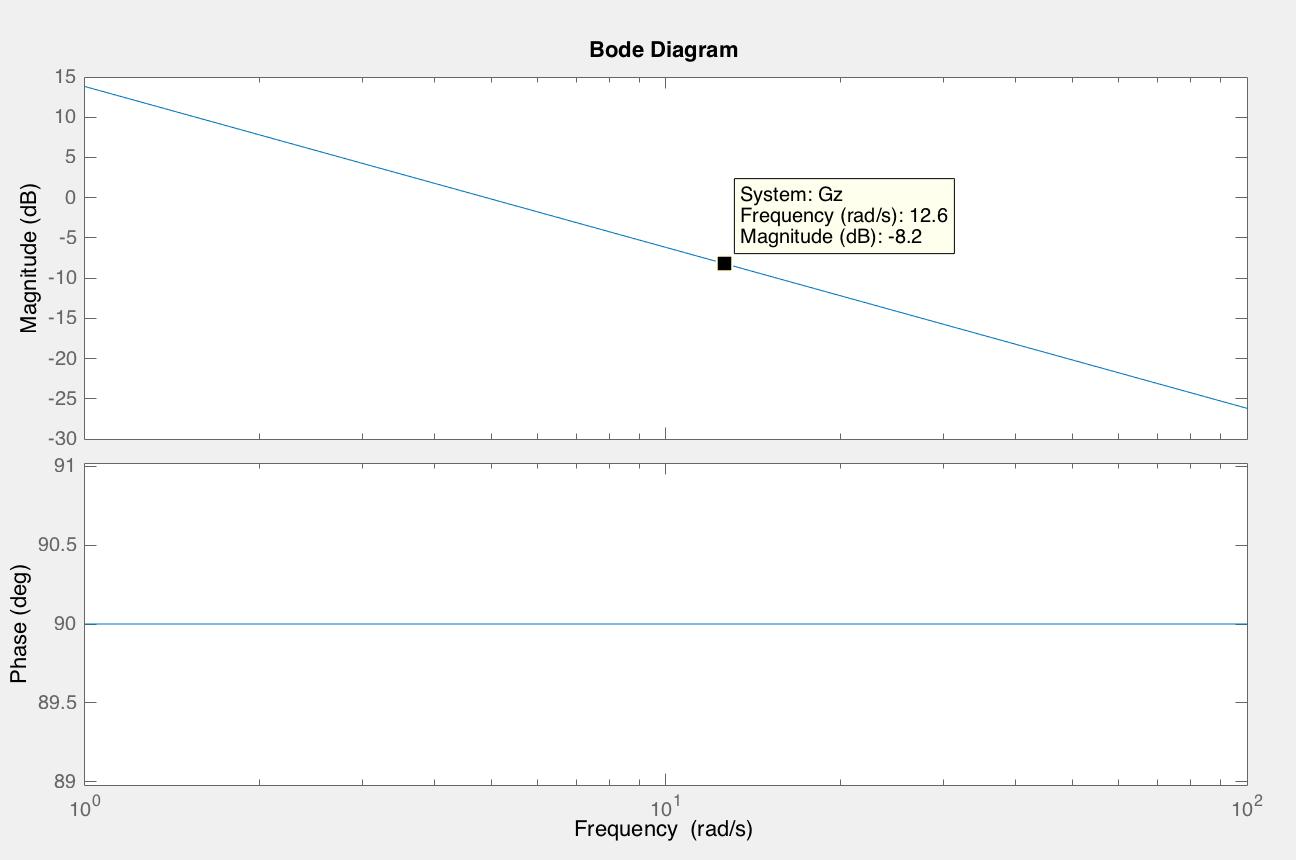
\includegraphics[width=0.7\textwidth]{figures/bode_z.png}
%	\caption{Bode plot of the plant with the 12.6 bandwidth displayed.}\label{fig:bode_z}
%\end{figure}
%The bode plot in \autoref{fig:bode_z} reveals that the magnitude is -8.2 dB at a magnitude of 12.6 rad/s. The magnitude has to be lifted by 5,2 dB to obtain the desired bandwidth. 
%
%The gain of the P-controller is found to be:
%\begin{align}
%C_y=10^{\frac{5.2}{20}}=1.82
%\end{align}
%The step response can be seen in

%
%The model expression for pitch is previously derived to be:
%\begin{align}
%m\Delta\ddot{y}_I = k_{th}({\overline{\omega}_1}^2+{\overline{\omega}_2}^2+{\overline{\omega}_3}^2+{\overline{\omega}_4}^2)\cos(\overline{\phi})\cos(\overline{\theta})\Delta\phi
%\label{eq:model_y_transl}
%\end{align}
%Laplace transforming \autoref{eq:model_y_transl_y} yields:
%\begin{align}
%m\cdot y_1(s)\cdot s^2= k_{th}\cdot (\omega_1 ^2 + \omega_2 ^2 + \omega_3 ^2 + \omega_4 ^2)\cdot \phi
%\end{align}
%The transfer function for the pitch is as follows:
%\begin{align}
%H_{y1}(s)=\frac{y_1(s)\cdot s}{\phi}=\frac{k_{th}\cdot (\omega_1 ^2 + \omega_2 ^2 + \omega_3 ^2 + \omega_4 ^2)}{m\cdot s}
%\end{align}
%\begin{where}
%\va{H_{y1}}{is the plant for the translational pitch}{1}
%\end{where}
